\documentclass[11pt,letterpaper]{article}

\usepackage[margin=1in]{geometry}
\usepackage{enumitem}
\usepackage{hyperref}
\usepackage{amsmath}
\usepackage{amssymb}
\usepackage{graphicx}
\usepackage{xcolor}
\usepackage{listings}

\lstset{
    language=Python,
    basicstyle=\ttfamily\footnotesize,
    keywordstyle=\color{blue!70!black}\bfseries,
    commentstyle=\color{green!40!black}\itshape,
    stringstyle=\color{red!60!black},
    numbers=left, numberstyle=\tiny\color{gray}, numbersep=6pt,
    frame=single, rulecolor=\color{gray!50},
    breaklines=true, showstringspaces=false, columns=fullflexible
}

\title{16.07 Dynamics\\Problem Set 2 --- Solutions}
\author{Due Monday, October 5}
\date{}

\newcommand{\bq}{\mathbf{q}}
\newcommand{\tq}{\tilde{\mathbf{q}}}
\newcommand{\bM}{\mathbf{M}}
\newcommand{\bC}{\mathbf{C}}
\newcommand{\bK}{\mathbf{K}}
\newcommand{\bR}{\mathbf{R}}
\newcommand{\bS}{\mathbf{S}}
\newcommand{\bI}{\mathbf{I}}
\newcommand{\ehat}{\hat{e}}
\newcommand{\nhat}{\hat{n}}
\newcommand{\uhat}{\hat{u}}
\newcommand{\Ou}{\Omega_u}
\newcommand{\On}{\Omega_n}

\begin{document}

\maketitle

\noindent\textbf{Notation.} Throughout, $s \equiv \sqrt{\ell^2 - x^2 - y^2}$ is the depth of the mass below the pivot, $\omega_0 \equiv \sqrt{g/\ell}$ is the pendulum frequency, and
\[
\On \equiv \Omega\cos\lambda, \qquad \Ou \equiv \Omega\sin\lambda
\]
are the north and up components of the Earth's angular velocity. We will also use the $2\times2$ skew-symmetric matrix
\[
\bS = \begin{bmatrix} 0 & -1 \\ 1 & 0 \end{bmatrix},
\qquad \bS^T = -\bS, \qquad \bS^2 = -\bI .
\]
Multiplying a vector by $\bS$ rotates it $90^\circ$ counterclockwise. Section~2 explains how $\bS$ relates to the skew-symmetric matrix $\mathbf{S}(\vec\omega)$ used for 3D rotations.
With $\ell = 10$~m and $g = 9.81$~m/s$^2$, $\omega_0 = 0.9905$~rad/s, and the swing period is $2\pi/\omega_0 = 6.34$~s.

\section{Deriving Equations of Motion}

\subsection*{(a) Energies}

The Earth's rotation axis lies in the plane spanned by $\nhat$ and $\uhat$ and makes angle $\lambda$ with the local horizontal (Fig.~1, left). So
\[
\vec\Omega = \Omega\cos\lambda\,\nhat + \Omega\sin\lambda\,\uhat
= \begin{bmatrix} 0 \\ \On \\ \Ou \end{bmatrix}_{\text{ENU}}.
\]
(Check: at the North Pole, $\lambda = 90^\circ$ and $\vec\Omega$ points straight up; at the equator, it points due north.)

Ignoring the translation of $P$, the inertial velocity of the mass is the velocity seen in the rotating frame plus the transport term:
\[
\vec v = \dot{\vec r} + \vec\Omega\times\vec r,
\qquad
\vec\Omega\times\vec r =
\begin{vmatrix} \ehat & \nhat & \uhat \\ 0 & \On & \Ou \\ x & y & z \end{vmatrix}
= (\On z - \Ou y)\,\ehat + \Ou x\,\nhat - \On x\,\uhat .
\]
The kinetic energy is
\[
T = \tfrac12 m|\vec v|^2 = \tfrac12 m\left[(\dot x + \On z - \Ou y)^2 + (\dot y + \Ou x)^2 + (\dot z - \On x)^2\right].
\]
Expanding and dropping the $\mathcal{O}(\Omega^2)$ terms,
\[
\boxed{T = \tfrac12 m\left(\dot x^2 + \dot y^2 + \dot z^2\right)
+ m\Ou\,(x\dot y - y\dot x) + m\On\,(z\dot x - x\dot z),
\qquad
U = m g z .}
\]

\paragraph{Why the $\mathcal{O}(\Omega^2)$ terms are negligible.} The dropped terms are centrifugal, of size $\sim\tfrac12 m\Omega^2\ell^2$, while the gravitational terms are $\sim mg\ell$. The ratio is $\Omega^2\ell/g \approx 5\times10^{-9}$. By contrast, the $\mathcal{O}(\Omega)$ (Coriolis) terms are down by only $\Omega/\omega_0 \approx 7\times10^{-5}$, and they act over tens of thousands of swings. They are what produce the precession.

\subsection*{(b) Eliminating the constraint}

Since the mass hangs below the pivot, $z < 0$, so we take the negative root:
\[
z = -\sqrt{\ell^2 - x^2 - y^2} = -s, \qquad
\dot z = \frac{x\dot x + y\dot y}{s}.
\]
Substituting, the $\On$ term becomes
\[
z\dot x - x\dot z = -s\dot x - \frac{x(x\dot x + y\dot y)}{s}
= -\frac{(\ell^2 - y^2)\,\dot x + x y\,\dot y}{s},
\]
using $s^2 + x^2 = \ell^2 - y^2$. The Lagrangian $L = T - U$ is
\[
\boxed{L = \tfrac12 m\left[\dot x^2 + \dot y^2 + \frac{(x\dot x + y\dot y)^2}{s^2}\right]
+ m\Ou\,(x\dot y - y\dot x)
- m\On\,\frac{(\ell^2 - y^2)\,\dot x + x y\,\dot y}{s}
+ m g s .}
\]

\subsection*{(c) Linearization via the Lagrangian}

Expand each term to second order in $(x, y, \dot x, \dot y)$, using
\[
s = \ell - \frac{x^2 + y^2}{2\ell} + \mathcal{O}(4), \qquad \frac1s = \frac1\ell + \mathcal{O}(2).
\]
\begin{itemize}
    \item $\tfrac12 m(\dot x^2 + \dot y^2)$ is already quadratic. The term $(x\dot x + y\dot y)^2/s^2$ is fourth order, so we drop it.
    \item $m\Ou(x\dot y - y\dot x)$ is already quadratic.
    \item $-m\On\left[(\ell^2 - y^2)\,\dot x + xy\,\dot y\right]/s = -m\On\ell\,\dot x + \mathcal{O}(3)$.
    \item $mgs = mg\ell - \dfrac{mg}{2\ell}(x^2 + y^2) + \mathcal{O}(4)$.
\end{itemize}
The quadratic Lagrangian is therefore
\[
L_2 = \tfrac12 m(\dot x^2 + \dot y^2) + m\Ou\,(x\dot y - y\dot x) - \frac{mg}{2\ell}(x^2 + y^2) - m\On\ell\,\dot x + \text{const}.
\]
The term $-m\On\ell\,\dot x$ is first order, but it will drop out in the Euler-Lagrange equation when we compute $\frac{d}{dt}\left(\frac{\partial L}{\partial \dot{x}}\right)$, so we drop it.

\paragraph{Equations of motion.}
\[
\frac{\partial L_2}{\partial\dot x} = m\dot x - m\Ou y, \quad
\frac{\partial L_2}{\partial x} = m\Ou\dot y - \frac{mg}{\ell}x
\quad\Longrightarrow\quad
m\ddot x - 2m\Ou\,\dot y + \frac{mg}{\ell}x = 0,
\]
\[
\frac{\partial L_2}{\partial\dot y} = m\dot y + m\Ou x, \quad
\frac{\partial L_2}{\partial y} = -m\Ou\dot x - \frac{mg}{\ell}y
\quad\Longrightarrow\quad
m\ddot y + 2m\Ou\,\dot x + \frac{mg}{\ell}y = 0.
\]
In the form $\bM\ddot\bq + \bC\dot\bq + \bK\bq = \mathbf 0$:
\[
\boxed{\bM = m\,\bI, \qquad
\bC = 2m\Omega\sin\lambda\begin{bmatrix}0 & -1\\ 1 & 0\end{bmatrix} = 2m\Ou\,\bS, \qquad
\bK = \frac{mg}{\ell}\,\bI.}
\]

\paragraph{Structure of $\bC$.} $\bC$ is \emph{skew-symmetric}: $\bC^T = -\bC$. Consequences:
\begin{itemize}
    \item $\dot\bq^T\bC\dot\bq = 0$, so the force $-\bC\dot\bq$ is always perpendicular to the velocity. It does no work and causes no damping.
    \item Only the vertical component $\Ou = \Omega\sin\lambda$ appears. For horizontal velocities, the horizontal component $\On\nhat$ produces a Coriolis force $-2m\On\nhat\times(\dot x\ehat + \dot y\nhat) = 2m\On\dot x\,\uhat$, which is vertical. That force is absorbed by the cable tension.
\end{itemize}

\section{Analyzing Precession}

Dividing Eq.~(1) by $m$ gives
\[
\ddot\bq + 2\Ou\bS\,\dot\bq + \omega_0^2\,\bq = \mathbf 0 .
\]
Take $\bR(\psi) = \begin{bmatrix}\cos\psi & -\sin\psi\\ \sin\psi & \cos\psi\end{bmatrix}$, which rotates counterclockwise by $\psi$, consistent with the definition of $\psi$. Let the frame rotate at a constant rate, $\psi(t) = \dot\psi\,t$.

\paragraph{Derivative of a rotation matrix.} Recall that in 3D, a rotation matrix $\bR(t)$ whose frame rotates with angular velocity $\vec\omega$ (expressed in the rotating frame) satisfies
\[
\dot\bR = \bR\,\mathbf{S}(\vec\omega),
\qquad
\mathbf{S}(\vec\omega) = \begin{bmatrix} 0 & -\omega_3 & \omega_2\\ \omega_3 & 0 & -\omega_1\\ -\omega_2 & \omega_1 & 0 \end{bmatrix},
\]
where $\mathbf{S}(\vec\omega)$ is the skew-symmetric matrix with $\mathbf{S}(\vec\omega)\,\mathbf{v} = \vec\omega\times\mathbf{v}$. The 2D case is the special case of rotation about a fixed axis perpendicular to the plane, $\vec\omega = [0\;\;0\;\;\omega]^T$. Keeping only the in-plane $2\times2$ block, $\mathbf{S}(\omega)$ depends on the single scalar $\omega$ and factors as
\[
\mathbf{S}(\omega) = \begin{bmatrix} 0 & -\omega\\ \omega & 0\end{bmatrix} = \bS\,\omega,
\qquad\text{so}\qquad
\dot\bR = \bR\,\mathbf{S}(\omega) = \bR\,\bS\,\omega .
\]
Here $\omega = \dot\psi$, so $\dot\bR = \bR\,\bS\,\dot\psi$. Unlike in 3D, every 2D rotation shares the same axis, so $\bS$ commutes with $\bR$: $\bS\bR = \bR\bS$. (You can also verify this directly by multiplying out the matrices.) These two facts make the algebra short.
Differentiating $\bq = \bR\tq$ twice:
\begin{align*}
\dot\bq &= \dot\bR\,\tq + \bR\,\dot{\tq} = \bR\left(\dot{\tq} + \bS\tq\,\dot\psi\right),\\
\ddot\bq &= \bR\,\bS\,\dot\psi\left(\dot{\tq} + \bS\tq\,\dot\psi\right) + \bR\left(\ddot{\tq} + \bS\dot{\tq}\,\dot\psi\right)
= \bR\left(\ddot{\tq} + 2\bS\dot{\tq}\,\dot\psi - \tq\,\dot\psi^2\right),
\end{align*}
where we used $\ddot\psi = 0$ and $\bS^2 = -\bI$. Substituting into the equation of motion:
\[
\bR\left[\ddot{\tq} + 2\bS\dot{\tq}\,\dot\psi - \tq\,\dot\psi^2\right]
+ 2\Ou\bS\bR\left[\dot{\tq} + \bS\tq\,\dot\psi\right]
+ \omega_0^2\bR\tq = \mathbf 0 .
\]
Moving $\bS$ past $\bR$, using $\bS^2 = -\bI$, and multiplying on the left by $\bR^T$:
\[
\boxed{\ddot{\tq} + 2\left(\dot\psi + \Ou\right)\bS\,\dot{\tq} + \left(\omega_0^2 - \dot\psi^2 - 2\Ou\dot\psi\right)\tq = \mathbf 0 .}
\]
The rotating frame contributes its own velocity-rotation term, $2\bS\dot{\tq}\,\dot\psi$, with the same structure as the Coriolis term. These two terms can cancel. (This step relies on $\bM$ and $\bK$ being multiples of $\bI$, so they commute with $\bR$. The linearized pendulum has no preferred horizontal direction.)

\subsection*{(a) Precession rate}

The $\bS\dot{\tq}$ term vanishes when
\[
\boxed{\dot\psi = -\Omega\sin\lambda .}
\]
With this choice, the remaining ODE is
\[
\ddot{\tq} + \left(\omega_0^2 + \Omega^2\sin^2\lambda\right)\tq = \mathbf 0
\;\approx\; \ddot{\tq} + \omega_0^2\,\tq = \mathbf 0,
\]
since $\Omega^2\sin^2\lambda/\omega_0^2 \lesssim 5\times10^{-9}$. (This is consistent with having dropped $\mathcal{O}(\Omega^2)$ terms in 1(a).) In the rotating frame, the mass behaves as an ordinary 2D pendulum. Its solutions $\tq(t)$ trace a fixed line or ellipse that does not rotate. Back in the Earth frame, $\bq = \bR(-\Ou t)\,\tq$ is that same fixed pattern turned steadily at rate $-\Ou$. So the swing plane precesses at $\dot\psi = -\Omega\sin\lambda$.

\subsection*{(b) Direction}

\begin{itemize}
    \item \textbf{Northern hemisphere} ($\lambda > 0$): $\dot\psi < 0$. Since $\psi$ is measured counterclockwise from above, the swing plane rotates \emph{clockwise} viewed from above. It rotates counterclockwise in the southern hemisphere.
    \item \textbf{Equator} ($\lambda = 0$): $\dot\psi = 0$, so there is no precession. $\vec\Omega$ is horizontal there, and horizontal rotation only produces vertical Coriolis forces on the (nearly horizontal) swing.
    \item \textbf{North Pole} ($\lambda = 90^\circ$): $\dot\psi = -\Omega$, one full clockwise turn per sidereal day. At the pole, the pivot is on the rotation axis and gravity is parallel to it, so nothing can exert a torque that rotates the swing plane in inertial space. The plane stays fixed relative to the stars while the Earth turns counterclockwise beneath it.
\end{itemize}

\subsection*{(c) Precession period at MIT}

With $\lambda = 42.36^\circ$, $\sin\lambda = 0.6737$:
\[
|\dot\psi| = \Omega\sin\lambda = 4.913\times10^{-5}~\text{rad/s} = 10.13^\circ/\text{h},
\qquad
T_{\text{prec}} = \frac{2\pi}{\Omega\sin\lambda} = 1.279\times10^5~\text{s} \approx \boxed{35.5~\text{h}.}
\]


\section{Simulation}

The code is listed at the end of this document. It integrates the linearized equations from 1(c) for 36~hours (just over one precession period, about 20{,}000 swings) using \texttt{solve\_ivp} with the \texttt{DOP853} method and relative and absolute tolerances of $10^{-10}$. The mass starts at rest with $x(0) = \ell\sin 5^\circ = 0.872$~m and $y(0) = 0$. (Because the equations are linear, starting from $\ell\theta_0$ instead gives identical precession.)

\paragraph{Energy check.} Because $\bC$ is skew-symmetric, the Earth-frame energy
\[
E = \tfrac12\dot\bq^T\bM\dot\bq + \tfrac12\bq^T\bK\bq
\]
is conserved exactly: $\dot E = \dot\bq^T(\bM\ddot\bq + \bK\bq) = -\dot\bq^T\bC\dot\bq = 0$. Over 36~hours, the maximum relative drift in $E$ was $8\times10^{-7}$, confirming the integration is accurate.

\paragraph{Computing $\psi$.} At each turning point (local maximum of $r = \sqrt{x^2 + y^2}$), the orientation of the swing line is computed as
\[
\psi = \tfrac12\,\texttt{atan2}\!\left(2xy,\; x^2 - y^2\right),
\]
which gives the angle of the line through the origin and $(x,y)$ modulo $\pi$. It does not care which end of the swing the mass is on. The $\pi$ jumps are then removed with $\psi_{\text{unwrapped}} = \tfrac12\,\texttt{unwrap}(2\psi)$. An equivalent approach is to use $\texttt{atan2}(y, x)$ and unwrap with a period of $\pi$.

\paragraph{Results.} Figure~\ref{fig:psi} shows the simulated $\psi(t)$ lying on top of the prediction. A linear fit gives
\[
\dot\psi_{\text{sim}} = -10.13445^\circ/\text{h}
\quad\text{vs.}\quad
\dot\psi_{\text{pred}} = -10.13445^\circ/\text{h},
\qquad
\text{error} \approx 6\times10^{-8}~\%.
\]
The agreement is at the level of numerical error.

\emph{Grading note:} Errors much larger than about $10^{-3}$\% usually indicate loose integration tolerances, too coarse an output time step (so the turning points are poorly located), or angle-wrapping mistakes. Visible jumps of $\pm180^\circ$ or $\pm90^\circ$ in $\psi(t)$ mean the unwrapping was not done with period $\pi$.

\begin{figure}[h]
\centering
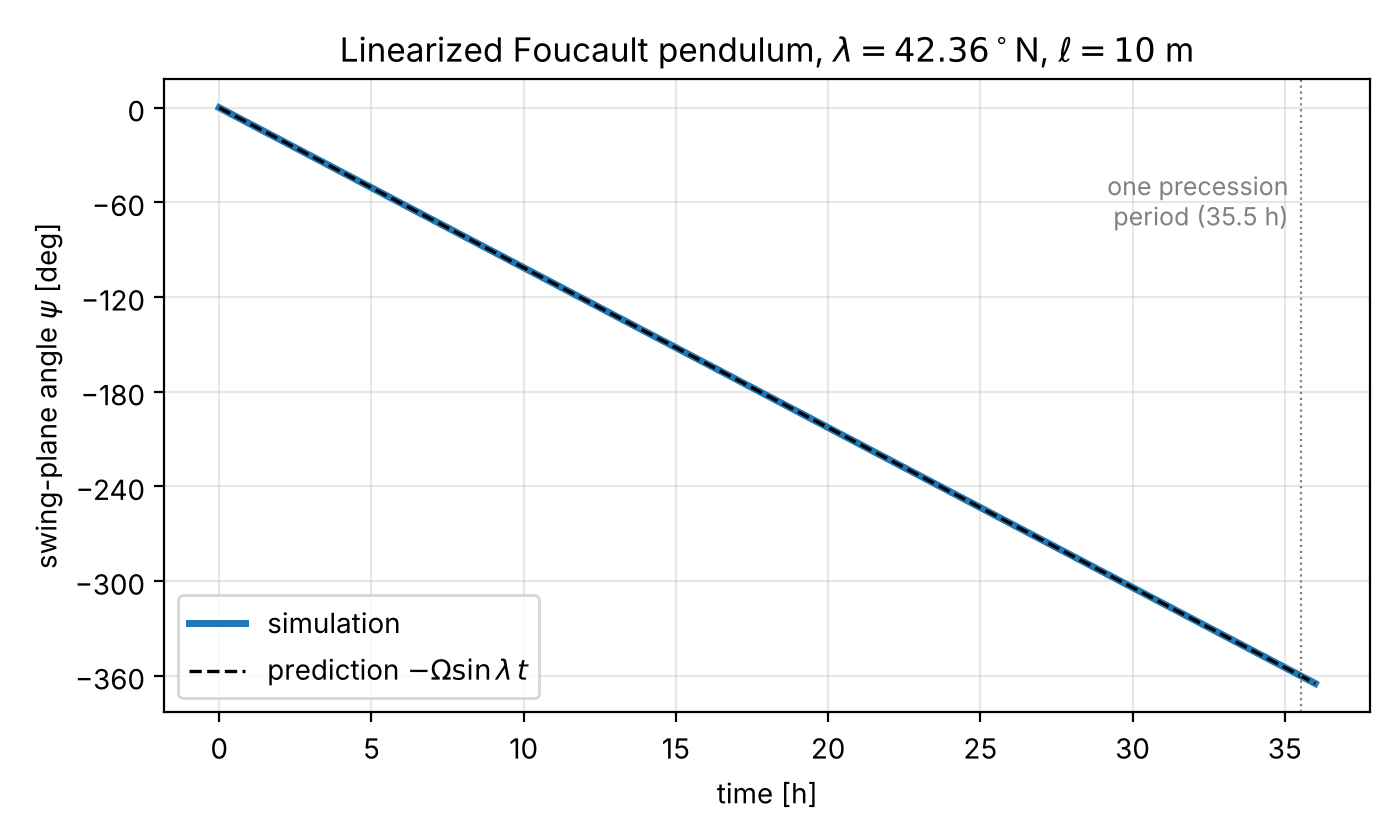
\includegraphics[width=0.8\textwidth]{psi_linear.png}
\caption{Simulated swing-plane angle $\psi$ (evaluated once per swing at the turning points) and the prediction $\psi = -\Omega\sin\lambda\,t$ for $\lambda = 42.36^\circ$N. The dotted line marks one precession period, 35.5~h.}
\label{fig:psi}
\end{figure}

\section*{Code}

\lstinputlisting{foucault_linear.py}

\end{document}
